\documentclass[12pt]{extarticle}
%Some packages I commonly use.
\usepackage[portuguese]{babel}
\usepackage{graphicx}
\usepackage{framed}
\usepackage[normalem]{ulem}
\usepackage{amsmath}
\usepackage{amsthm}
\usepackage{amssymb}
\usepackage{amsfonts}
\usepackage{enumerate}
\usepackage[utf8]{inputenc}
\usepackage{float}
\usepackage{gensymb}
\usepackage[top=1 in,bottom=1in, left=1 in, right=1 in]{geometry}
\usepackage{multirow}
\usepackage{caption}
\usepackage{subcaption}
\usepackage[utf8]{inputenc}


%A bunch of definitions that make my life easier
\newcommand{\matlab}{{\sc Matlab} }
\newcommand{\cvec}[1]{{\mathbf #1}}
\newcommand{\rvec}[1]{\vec{\mathbf #1}}
\newcommand{\ihat}{\hat{\textbf{\i}}}
\newcommand{\jhat}{\hat{\textbf{\j}}}
\newcommand{\khat}{\hat{\textbf{k}}}
\newcommand{\minor}{{\rm minor}}
\newcommand{\trace}{{\rm trace}}
\newcommand{\spn}{{\rm Span}}
\newcommand{\rem}{{\rm rem}}
\newcommand{\ran}{{\rm range}}
\newcommand{\range}{{\rm range}}
\newcommand{\mdiv}{{\rm div}}
\newcommand{\proj}{{\rm proj}}
\newcommand{\R}{\mathbb{R}}
\newcommand{\N}{\mathbb{N}}
\newcommand{\Q}{\mathbb{Q}}
\newcommand{\Z}{\mathbb{Z}}
\newcommand{\<}{\langle}
\renewcommand{\>}{\rangle}
\renewcommand{\emptyset}{\varnothing}
\newcommand{\attn}[1]{\textbf{#1}}
\theoremstyle{definition}
\newtheorem{theorem}{Theorem}
\newtheorem{corollary}{Corollary}
\newtheorem*{definition}{Definition}
\newtheorem*{example}{Example}
\newtheorem*{note}{Note}
\newtheorem{exercise}{Exercise}
\newcommand{\bproof}{\bigskip {\bf Proof. }}
\newcommand{\eproof}{\hfill\qedsymbol}
\newcommand{\Disp}{\displaystyle}
\newcommand{\qe}{\hfill\(\bigtriangledown\)}
\setlength{\columnseprule}{1 pt}
\usepackage[utf8]{inputenc}

\title{Aceleração e Movimento Uniformemente Variado (MUV)}
\author{Felipe Salvador}
\date{Atualizado em \today}

\begin{document}

\maketitle

Na aula de hoje, iremos dar continuidade ao assunto de cinemática, para explorar o que é a aceleração e entender um outro tipo de movimento: o Movimento Uniformemente Variado (MUV). Vamos partir dos conceitos da aula passada de velocidades e do Movimento Retíílineo Uniforme (MRU) para construir um outro conceito mais geral.

\section{Aceleração (a)}

Na aula passada, vimos o conceito de \textbf{velocidade}: uma quantidade que nos diz a distância que percorremos dentro de um intervalo de tempo. Ela é explicitamente dita por:

\begin{equation}
    v = \frac{\Delta S}{\Delta t},
\end{equation}
em que $\Delta S$ é a distância percorrida e $\Delta t$ é o intervalo de tempo levado para percorrer essa distância $\Delta S$. Vimos que essa velocidade nos diz o quão rápido estamos nos movendo no espaço e o sinal dela depende para onde estamos indo. \textbf{Se estamos indo em direção à origem do espaço (o 0), então a velocidade é negativa. Caso estejamos nos afastando da origem, a velocidade é positiva.}

Porém, tem um detalhe muito importante que deixamos passar na aula passada. É que essa velocidade da equação (1) é uma \textbf{velocidade constante}, ou seja, é uma velocidade que não muda. Bem, isso não descreve tudo que acontece na Cinemática, porque um carro pode freiar ou acelerar e isso faz mudar a velocidade dele.

\begin{figure}[H]
    \centering
    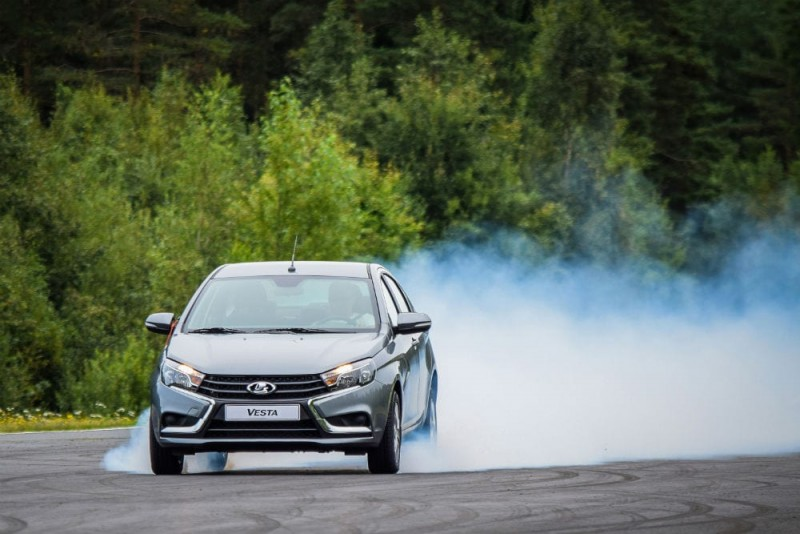
\includegraphics[width = 0.5\textwidth]{economizar-combustivel-evite-frear-e-acelerar-bruscamente.jpg}
    \caption{Imagem de um carro freiando. Na frenagem, a velocidade do carro diminui, podendo até parar.}
    \label{fig:brake}
\end{figure}

Com isso, precisamos de uma quantidade que descreve o quanto a velocidade mudou dentro de um intervalo de tempo. O nome que damos a essa quantidade chama-se \textbf{aceleração} e é descrita da seguinte forma:

\begin{equation}
    a= \frac{\Delta v}{\Delta t} = \frac{v_f - v_i}{\Delta t}
\end{equation}
em que $\Delta v$ é a variação de velocidade dentro de um intervalo de tempo e ela é dada por: $\Delta v = v_f - v_i$, tal que $v_f$ é a velocidade final e $v_i$ é a velocidade inicial.

O que essa quantidade nos diz é que dado um intervalo de tempo que eu vou observar o movimento e dados a velocidade do objeto no início da medição ($v_i$) e a velocidade do objeto no final da medição ($v_f$), eu consigo determinar quanto a velocidade variou num intervalo de tempo.

A unidade da aceleração([a]) é dada por:

\begin{equation}
    [a] = \frac{[v]}{[t]} = \frac{\frac{m}{s}}{s} = \frac{m}{s*s} \implies [a] = \frac{m}{s^2}
\end{equation}
lê-se: \textit{metro por segundo ao quadrado}.

Vamos tentar entender como funciona essa quantidade em exemplos.

\begin{itemize}
    \item \textit{Exemplo 1:} Um carro na Rodovia Presidente Dutra está andando à 30 m/s. O motorista vê um congestionamento a frente dele e pisa no freio a fim de parar o carro. Após 6s, o carro para completamente. Qual é a aceleração que o carro sofreu?
    
    Primeiramente, vamos entender quais são as informações do enunciado. O carro andava à 30 m/s, então essa é a velocidade inicial: $v_i = 30 m/s$.
    
    No segundo instante (t=6s), o carro parou completamente, ou seja, $v_f =0 m/s$. Tudo isso ocorreu num intervalo de tempo de $\delta t = 6s$.
    
    Logo, temos todas as informações para o exemplo:
    
    \begin{align*}
        &a = \frac{\Delta v}{\Delta t} = \frac{v_f - v_i}{\Delta t} \\ &a = \frac{0 - 30}{6}
    \end{align*}
    \begin{align}
        \boxed{ a = - 5 m/s^2}
    \end{align}
    
    \textbf{Sempre que falarmos de 'freiar', a aceleração é negativa e quando falarmos de 'acelerar', a aceleração é positiva. Cuidado para não confundir o termo da física com o popular!!!}
    
    \item \textit{Exemplo 2:} Uma forma de verificar a potência de um carro é medir em quantos segundos um carro demora para ir de 0 a 100 km/h. Num teste realizado pela revista QuatroRodas com os carros Fiat Uno Attractive 1.0 e Fiat Uno Fire 1.3, os carros foram de 0 a 100 km/h em 15.6 s e 12.5 s, respectivamente.
    
    Quais foram as acelerações dos carros nesse teste?
    
    Bem, antes de fazermos qualquer conta, prestemos atenção às informações dadas e suas unidades. Perceba que o teste é saber o  tempo que o carro leva para $v_i = 0$ km/h para $v_f = 100$ km/h e que o tempo medido é dados em segundos. Então, as unidades não são equivalentes, então temos que transformar uma das 2 unidade para podermos trabalhar.
    
    Aqui, vamos transformar a velocidade, porque transformar o tempos em segundos, que tá na forma decimal, para horas requer uma conta meio chatinha de se fazer. Logo, lembremos que:
    
    \begin{align}\label{eq:transf}
        \frac{m}{s} \xrightarrow{x\, 3.6} \frac{km}{h} \quad \quad \quad \frac{km}{h} \xrightarrow{\div\, 3.6} \frac{m}{s}
    \end{align}
    
    Então:
    
    \begin{align*}
        &v_i: \, 0 km/h \div 3.6 = 0 m/s \\
        &v_f: \, 100 km/h \div 3.6 = 27,8 m/s
    \end{align*}
    
    Agora, temos todas as informações em unidades que podemos trabalhar sem nos preocupar em misturar unidades. Pela equação (1), a aceleração do carro Uno Attractive 1.0 ( $a_{1.0}$) e do Uno Fire 1.3 ($a_{1.3}$):
    
    \begin{align*}
        &a_{1.0} = \frac{\Delta v}{\Delta t} = \frac{v_f - v_i}{\Delta t} = \frac{27,8 - 0}{15,6} \\
        & a_{1.3} = \frac{\Delta v}{\Delta t} = \frac{v_f - v_i}{\Delta t} = \frac{27.8 - 0}{12.5}
    \end{align*}
    Finalmente, temos que:
    
    \begin{align}
        \boxed{a_{1.0} \approx 1,8 m/s^2 \quad \quad
        a_{1.3} \approx 2,2 m/s^2}
    \end{align}
    \end{itemize}
    
    \section{Movimento Uniformemente Variado (MUV)}
    
    A classe de movimento retilíneo mais geral é a do Movimento Uniformemente Variado (MUV), porque ela não depende de que a velocidade seja constante, mas ao custo de que exista uma aceleração constante no problema. Então, a partir disso, podemos achar a posição do objeto para um dado tempo, mas precisamos de 2 informações iniciais para podermos determinar a posição com precisão.
    
    Vamos partir da equação da aceleração (equação (1)):
    
    \begin{align*}
        a = \frac{\Delta v}{ \Delta t} = \frac{v - v_0}{t - t_0}
    \end{align*}
    Aqui, chamamos de $v$ a velocidade no tempo $t$, $v_0$ a velocidade inicial do objeto (equivalente ao $v_i$) e $t_0$ o tempo inicial de quando o movimento começou. O tempo inicial é algo que eu possa escolher de onde começa e, para não causar problemas, colocamos sempre $t_0 =0$. Portanto:
    
    \begin{align*}
        &a = \frac{v - v_0}{t} \\
        & at = v - v_0
        \end{align*}
        \begin{align}\label{eq:velocidade}
        v = v_0 + at  
        \end{align}
        
        Essa última equação é a \textbf{equação da velocidade.} Ela que nos diz a velocidade num certo tempo $t$, para uma dada aceleração $a$ e uma velocidade inicial $v_0$.
        
        Existe também uma fórmula para a posição do corpo, que é dada por:
        
        \begin{align}\label{eq:sorvetao}
            S = S_0 + v_0*t + \frac{at^2}{2}
        \end{align}
        
        \textbf{Essa é a função horária do espaço para o MUV.} A dedução dessa fórmula, nós veremos no final do conteúdo de cinemática, quando falaremos de gráficos. Essa fórmula é também conhecida como \textbf{fórmula/equação do Sorvetão.}
        
        Quando a aceleração do movimento MUV é positiva, nós dizemos que o movimento é uniformemente acelerado ou movimento acelerado. Caso contrário, o movimento é dito movimento retrógado.
        
        Toda a discussão aqui feita também é válida para o movimento vertical. Nesse caso, a aceleração sempre será a aceleração da gravidade (g): $g\approx 9.8 m/s^2$. Esse tipo de problema são os problemas de \textbf{queda livre.}
        
        \begin{itemize}
            \item \textit{Exemplo 1:} Uma razão para a diminuição da velocidade nas vias expressas da Marginal Pinheiros e Tietê é a redução de acidentes. Um indicativo de acidente é o número de batidas entre carros, especialmente as batidas traseiras. Uma das causas das batidas traseiras é quando o carro de trás não consegue parar a tempo e bate no carro da frente parado. 
            
            Então, calculou o espaço percorrido por um carro numa frenagem de 3s. Um frenagem forte tem aceleração da ordem de $2 m/s^2$. Então, um carro a 20 m/s (72 km/h) na Marginal Pinheiros precisa freiar para não colidir com um carro parado na via. 
            
            Qual é a distância mínima em relação ao carro parado que o carro em movimento tem que começar a freiar para não colidir?
            
            As informações do enunciado são as seguintes: tempo de frenagem: $t=3s$; aceleração/desaceleração do carro: $a = 2m/s^2$; velocidade inicial: $v_0 = 20m/s$. 
            
            O exercício quer a distância mínima para não bater, ou seja, qual é a distância que o carro percorre na frenagem para parar.
            
            Aqui vamos usar a equação(\ref{eq:sorvetao}) para achar a distância. A fórmula precisa da informação da posição inicial do carro em movimento ($S_0$), mas como ele não deu, podemos assumir que $S_0=0$. \textbf{Como é uma frenagem, a aceleração é negativa}. Logo, a fórmula fica:
            
            \begin{align*}
                &S = S_0 + v_0*t + \frac{at^2}{2} \\
                & S = 0 + 20*3 + \frac{-2*3^2}{2}\\
                & S = 60 + -\frac{-2*9}{2} \\
                & S = 40 - 9\\
            \end{align*}
            Logo:
            \begin{align}
                \boxed{S = 31 m}
            \end{align}
            A distância mínima que o carro em movimento tem que começar a freiar é de 31 m em relação ao carro parado. Isso quer dizer que o carro anda 31 metros até ele parar completamente.
            
            \
            \item \textit{Exemplo 2: Continuação do exemplo 1 de aceleração} - Agora, com o resultado de aceleração obtido, vamos calcular qual é a distância que os Unos percorrem até os 100 km/h.
            
            Nesse exemplo, vamos usar os tempos que os carros levam e as acelerações que obtivemos. $t_{1.0},\, a_{1.0}$ são o tempo e a aceleração que o Uno 1.0 teve; $t_{1.3},\, a_{1.3}$ são o tempo e aceleração que o Uno 1.3 teve. Usando a equação do Sorvetão (eq. (\ref{eq:sorvetao})) para fazer os cálculos. Vamos supor que ambos os carros estão na origem em $t=0$ e que estão parados $V_0=0$ Logo:
            
            \begin{align*}
                &t_{1.0} = 15.6 s &  & t_{1.3} = 12.5 s \\
                &a_{1.0} \approx 1.8 m/s^2 & & a_{1.3} \approx 2.2 m/s^2 \\
                & S_{1.0} = \underbrace{S_0}_{=0} + \underbrace{V_0}_{=0}* t + \frac{a_{1.0}*t^2}{2} & & S_{1.3} = \underbrace{S_0}_{=0} + \underbrace{V_0}_{=0}* t + \frac{a_{1.3}*t^2}{2}  \\
                & S_{1.0} = \frac{1,8*15,6^2}{2} & & S_{1.3} = \frac{2.2*12.5^2}{2} \\
            \end{align*}
            
            Fazendo as contas na calculadora, temos que:
            
            \begin{align}
                \boxed{S_{1.0}\approx 219,0m \quad \quad S_{1.3}\approx 171,9m}
            \end{align}
            
            Ou seja, o Uno 1.3 percorre um espaço menor até atingir 100km/h do que o Uno 1.0.
        \end{itemize}
        
        \section*{LISTA DE EXERCÍCIOS}
        \textit{Obs - caso necessário, use a relação da eq.(\ref{eq:transf}) para transformar km/h para m/s ou vice-versa}
        
        \begin{enumerate}
            \item Um objeto realiza um movimento acelerado de modo que a sua velocidade passa a ser de 30 m/s em que o objeto partiu do repouso e demorou 5s para atingir essa velocidade. Qual é a aceleração média desse corpo?
            \begin{enumerate}
                \item $2,5 m/s^2$;
                \item $0,5 m/s^2$;
                \item $1,0 m/s^2$;
                \item $5,0 m/s^2$;
                \item $6,0 m/s^2$;
            \end{enumerate}
            
            \item As faixas de aceleração das auto-estradas devem ser longas o suficiente para permitir que um carro, partindo do repouso, atinja a velocidade escalar de 100 km/h em 18s. Suponha que a aceleração escalar seja constante determine (\textit{assuma que o carro parta da origem}):
            \begin{enumerate}
                \item o valor da aceleração;
                \item a distancia percorrida em 10s;
                \item o comprimento mínimo da faixa de aceleração;
            \end{enumerate}
            
            \item  O recordista mundial dos 100m rasos cumpriu o percurso num intervalo de tempo próximo a 10s. Se o movimento do corredor fosse uniformemente acelerado a partir do repouso e durante toda a corrida, sau velocidade escalar no instante da chegada seria próxima de:
            \begin{enumerate}
                \item 72 km/h;
                \item 54 km/h;
                \item 36 km/h;
                \item 18 km/h;
                \item 10 km/h;
            \end{enumerate}
            
            \item Um carro partindo do repouso, assume movimento com aceleração contante de 1m/s durante 5 segundos. Desliga-se então o motor e, devido ao atrito, o carro volta ao repouso com retardamento constante de 0,5m/s. A duração total do movimento do corpo é de?
            
            \begin{enumerate}
                \item 5s;
                \item 10s;
                \item 15s;
                \item 20s;
                \item 25s;
            \end{enumerate}
            
            \item Numa competição automobilistica, um carro se aproxima de uma curva em grande velocidade.O piloto, então, pisa no freio durante 4s e consegue reduzir a velocidade do carro para 30m/s.Durante a freada o carro percorre 160m.Supondo que or freios imprimam ao carro uma aceleração retardada constante.Calcule a velocidade do carro no instante em que o piloto pisou no freio.
            
            \item Um ciclista A inicia uma corrida a partir do repouso, acelerando $0,50 m/s^2$. Nesse instante, passa por ele outro ciclista B, com velocidade constante de 5,0 m/s e no mesmo sentido que o ciclista A. Determine:
            
            \begin{enumerate}
                \item Quanto tempo após a largada A alcança B.
                \item A distância percorrida por A para alcançar B.
                \item A velocidade de A no instante que alcança B.
            \end{enumerate}
        
        \item Um objeto é lançado, verticalmente para cima, do topo de um prédio com altura $h=50 m$ e a velocidade inicial do objeto é de $v_0 = 15 m/s$. Quanto tempo demora para o objeto chegar ao chão e qual é a velocidade que ele atinge o chão. \textit{Obs: aceleração da gravidade $g=10 m/s^2$}:
        
        \textit{Caso necessite, a fórmula para resolver equação de segundo grau é ($ax^2 +bx+c=0$): $x = \frac{-b \pm \sqrt{\Delta}}{2*a}$, em que $\Delta = b^2 - 4*a*c$}
        \begin{enumerate}
            \item $t=2,0$ e $v=5m/s$;
            \item $t=2,0$ e $v=-5m/s$;
            \item $t=5,0$ e $v=-35m/s$;
            \item $t=5,0$ e $v=35m/s$;
        \end{enumerate}
        \end{enumerate}
        
        \pagebreak
        
        \section*{GABARITO}
        
        \begin{enumerate}
            \item (e)
            \item
            \begin{enumerate}
                \item $a=1.53 m/s^2$
                \item Após 10 s, $\Delta S =76,5m$
                \item A faixa deve ter o tamanho de $\Delta S = 247,85 m$
            \end{enumerate}
            
            \item (a)
            \item (c)
            \item $v_0 = 50 m/s$
            \item \begin{enumerate}
                \item $t = 20s$
                \item $\Delta S = 100m$
                \item $v = 10 m/s$
            \end{enumerate}
            
            \item (c)
        \end{enumerate}
\end{document}
